%!TEX root = thesis.tex"`

\chapter{Автоматизация и версионирование экспериментов}
В развитии большинства \acrshort{ml}-проектов наступает момент перехода от стадии экспериментирования с прототипом модели к стадии построения системы, обладающей способностью к автоматическому запуску, наблюдаемостью и возможностью отслеживания ошибок. 
Данный процесс может быть весьма сложен, поскольку включает в себя применение некоторых практик \gls{swe} и \gls{devops}.
Его изложению и будут посвящены дальнейшие секции.
\section{Технический долг в \acrshort{ml} системах}
\label{sec:ml-debt}
В статье \cite{cite:ml-debt} подробно описан так называемый технической долг в применении к \acrshort{ml}-проектам.
Многие из указанных авторами проблем были характерны и для настоящей работы:
\begin{enumerate}
    \item Зависимость от нестабильных данных.
        Данные, используемые во всем процессе или отдельных экспериментах, могут храниться в ненадежном месте или не быть доступными воспроизводимым способом.
    \item Отсутствие статических проверок на наличие данных.
        Подразумевается проверка на наличие всех необходимых данных перед запуском каждой стадии процесса.
    \item <<Спагетти-код>> -- основной код перемешан с большим количеством связывающего кода, не несущего существенного смысла, но необходимого для соединения компонент воедино.
    \item Тупиковые экспериментальные ветвления, при которых в коде присутствует множество ответвлений для некоторых экспериментов, которые были заброшены и в актуальной версии кода приводят соответствующее ответвление в нерабочее состояние.
    \item Отсутствие отслеживания конфигурации всего \gls{pipeline}.
    Настройки модели должны быть явно выделены, должны версионироваться и быть простыми для визуального понимания человеком.
    \item Мониторинг и тестирование.
        Модель и \gls{pipeline} должны иметь систему журналирования действий, систему отслеживания ошибок и отклонений от ожидаемого поведения.
    \item Воспроизводимость.
        Каждый разработчик должен быть в состоянии воспроизвести то же состояние \gls{pipeline}, что и другой разработчик, с теми же выходными данными и состоянием кода.
    \item Слабая способность к управлению множественными процессами.
        При запуске большого количества моделей должна быть возможность следить за каждой из них с учетом описанных выше требований.
\end{enumerate}
Каждая из этих проблем была решена в рамках настоящей работы.
Изложению способа решения и достигнутых результатов будут посвящены дальнейшие главы.
\section{Автоматизация \gls{pipeline} обучения}
Выстраивание системы автоматического запуска всех шагов процесса обучения -- одна из первых задач на пути решения описанных в \ref{sec:ml-debt} проблем.
Для построения автоматизации такого рода был выбран фреймворк \gls{dvc} \cite{cite:dvc}.
На момент написания данной работы была актуальна версия 2.10.2, и дальнейшее изложение будет строиться на основе нее.

\Gls{dvc} оперирует в абстракциях <<стадий>> (\textit{stage}) -- некоторых действиях над данными.
Каждая такая стадия имеет входные данные (\textit{deps}), выходные данные (\textit{outs}), параметры, от которых стадия зависит (\textit{params}), и опционально может содержать метрики (\textit{metrics}) и графики (\textit{plots}).
Основная идея состоит в том, чтобы каждая стадия была зависима либо от выхода предыдущей стадии, либо от <<сырых>> данных, явно прописанных как часть \gls{pipeline}.
При таком подходе становится возможным представить весь процесс работы \acrshort{ml}-проекта как проход по \textit{направленному ацикличному графу}, называемому также \acrfull{dag}.
Визуальная иллюстрация приведена на рисунке \ref{fig:dvc-pipeline}.

\begin{figure}[!h]
    \centering
    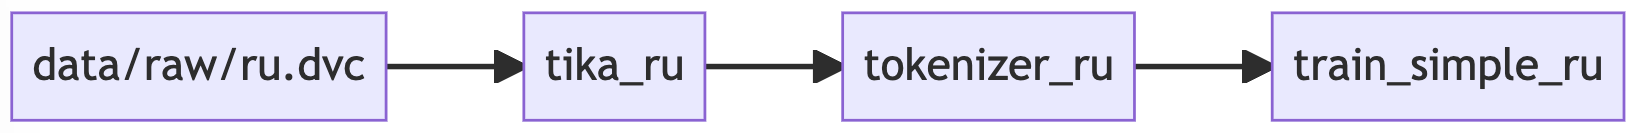
\includegraphics[width=\linewidth]{dvc-pipeline}
    \caption{Визуальное представление \acrshort{dag} обучения}
    \label{fig:dvc-pipeline}
\end{figure}

Приведенный на рисунке \ref{fig:dvc-pipeline} граф был построен по следующим правилам:
\begin{enumerate}
    \item Каждая стадия и каждый явно прописанный входной файл представляются вершинами графа.
    \item Для каждой стадии анализируется список ее зависимостей (\textit{deps}).
        Если эти зависимости удовлетворяются одной из описанных стадий (проверются выходные файлы стадии) или входным файлом, указанном наравне со стадиями, то проводится ребро между двумя стадиями, направленное в стороне зависимой.
        Если зависимости не удовлетворяются, то выдается ошибка запуска.
    \item Проверяется наличие циклов в полученном графе.
        Если они обнаружены, то выдается ошибка запуска.
\end{enumerate}
Построенный таким образом граф не только задает последовательность операций, но и явно описывает все входные и выходные данные.
Это позволяет настроить \textit{статистические проверки на наличие данных}, которые описаны среди проблем в \ref{sec:ml-debt}.
Помимо этого, описание всего процесса в едином графе вычислений дает возможность управлять процессом и производить его масштабирование, добавляя тем самым \textit{способность к управлению множественными процессами}.

Разделение кода на стадии, предлагаемое в \gls{dvc}, позволяет выстроить четкое разделение процесса на состоявляющие компоненты, избавляя от описанной в \ref{sec:ml-debt} проблемы <<спагетти>>-кода: вместо единого большого файла с набором инструкций будет порождено несколько небольших скриптов, выполняющих одну задачу, и выполняющих ее хорошо.
В настоящей работе удалось успешно осуществить такое разделение.
Первональная версия модели, выполненная в едином файле \gls{jupyter-notebook}, была разбита на множество отдельных скриптов, каждый из которых расширял и обобщал существующую функциональность исходного прототипа.
\section{Версионирование данных, артефактов и визуализация метрик}
% TODO: (ruapyyj) ну, тоже dvc <- Tue Apr 26 23:11:29 2022
\label{sec:dvc}
\section{Будущие автоматизации процесса}
% TODO: (ruapyyj) gitlab ci нормальный, CML, валидация данных (распределения), автоматическое детектирование серьезных ошибок <- Tue Apr 26 23:12:12 2022
